\chapter{Low Frequency Radio Astronomy and the Earth's Ionosphere}\label{Ch:Iono}


\section{Overview}

Beyond the effects of RFI, the Earth's atmosphere has additional impacts on low frequency radio signals from the universe. These impacts come from interactions between the incoming radio signals and free electrons in the ionosphere. Impacts include refraction and absorption at radio frequencies. 

Ionospheric impacts can mask the \cm signal by introducing additional frequency dependent structure into the sky signal. This frequency structure is proportional to $\nu^{-2}$, as explained below, and may be larger than the \cm structure for the SCI-HI frequency band. In addition, ionospheric structure is time and latitude dependent. Therefore, it is necessary to quantify and address ionospheric impacts to any \cm measurement. 

\begin{figure}[htb]
\centering
%\begin{minipage}[b]{0.48\textwidth}
%\centering
%\begin{tabular}{|c|c|}
%\hline
%Layer & Altitude Range (km) \\
%\hline
%D & 60-100 \\
%\hline
%E & 100-150 \\
%\hline
%F1 & 150-250 \\
%\hline
%F2 & 250-600 \\
%\hline
%topside & 600 - 1000+ \\
%\hline
%\end{tabular}
%\caption{Average altitudes and distribution of the Earth's ionosphere layers.}
%\label{Tab:iono_layer}
%\vspace{2cm}
%\end{minipage}%
%\begin{minipage}[b]{0.02\textwidth}
%\hspace{1cm}
%\end{minipage}%
%\begin{minipage}[b]{0.48\textwidth}
%\centering
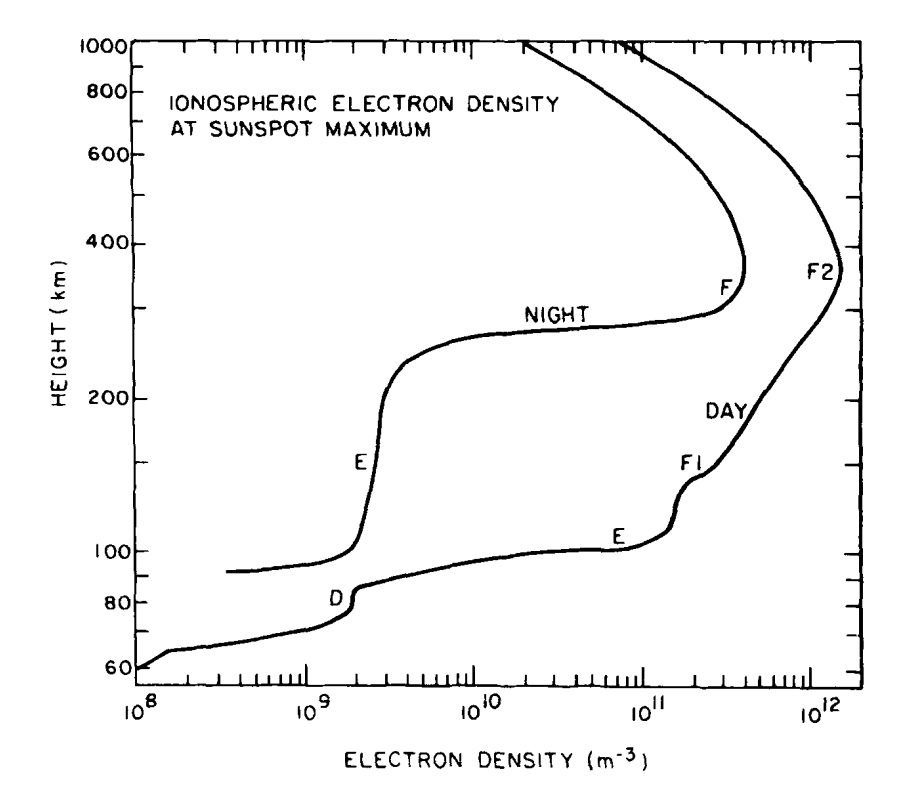
\includegraphics[width=0.95\linewidth]{Ionosphere/figures/atmosphere_layers.jpg}
\caption{Idealized average free electron density distribution in Earth's atmosphere. Layers are shown during day and night. Each layer corresponds to an inflection point in the free electron density distribution, referred to in the literature as a maximum. }
\label{Fig:iono_layer}
%\end{minipage}
\end{figure}



\section{Earth's Ionosphere}

To understand ionospheric impacts on the \cm signal we need to understand the ionosphere. Earth's ionosphere is located $60 - 1000+$ $km$ above the surface of the Earth and is made up of free electrons and ionized atoms. Neutral atoms in Earth's atmosphere are photoionized by solar radiation, which leads to an altitude dependent distribution of free electrons and ions in the atmosphere.


\subsection{Ionosphere Layers}

We can separate the ionosphere into altitude-dependent layers based on the distribution of free electrons. Each layer is defined by an altitude where the free electron distribution has an inflection point, commonly described in the literature as a local maximum. The altitude corresponding to the inflection point is the center altitude of the layer. Depending on the time of day and geographic location, the number of layers present in the ionosphere will vary as shown in Figure \ref{Fig:iono_layer}. There are four layers defined using inflection points (D, E, F1 and F2). A fifth topside layer is defined as the altitude above the F2 layer where the dominant ion in the ionosphere becomes $O^+$. The absolute maximum free electron density ($n_e$) is reached in the F2 layer and is $n_e \cong 10^5 cm^{-3}$ \cite{ionospheres}. 

Earth's ionosphere comes from solar radiation photoionizing neutral atoms, which is balanced by recombination of ions and free electrons. This ionization and recombination balance leads to fluctuations in the free electron density and ionospheric layers that depend on the amount of solar radiation currently impacting a given latitude and longitude. There are three major sources of variability in solar radiation levels that affect the ionosphere \cite{ionospheres}.

First, solar radiation is maximized during daylight. During those times, the free electron density is large, and more ionospheric layers are present (see Figure \ref{Fig:iono_layer}). In contrast, there is little to no solar radiation at night, so fewer ionospheric layers are present \cite{ionospheres}. 

Second, solar radiation levels are also always much lower at polar latitudes than they are at mid-latitudes. This is due to the lower sun angle at polar latitudes. During the polar winter, solar radiation levels and the number of free electrons in the atmosphere reach a minimum \cite{ionospheres}. 

Third, solar radiation levels have a periodic cycle of $\sim 11$ years as tracked by sunspot frequency. During a period of high sunspot activity, the corresponding levels of solar radiation are also higher, leading to larger free electron density \cite{ionospheres}. 


\subsection{Ionosphere Properties}

\subsubsection{Plasma Frequency}

Free electrons in the ionosphere can be treated as a plasma which modifies electromagnetic wave propagation. Change in propagation due to a plasma is quantified using the plasma frequency ($\nu_p$), which has a value given in Equation \ref{Eq:nu_p}, where $n_e$ is in $m^{-3}$ \cite{thompson_2001}. 

\begin{equation} \label{Eq:nu_p}
\nu_p = \frac{e}{2 \pi} \sqrt{\frac{n_e}{\varepsilon_0 m}} \cong 9 \sqrt{n_e} Hz
\end{equation}

This plasma frequency changes the index of refraction for the ionosphere compared to free space ($n = \sqrt{1-\nu_p^2/\nu^2}$), where $\nu$ is the frequency of the radiation that is passing through the atmosphere. The plasma frequency is typically $\nu_p \leq 12 MHz$, below the SCI-HI frequency band. Above the plasma frequency, electromagnetic waves are refracted by the ionosphere. Meanwhile, below the plasma frequency the ionosphere reflects electromagnetic waves, preventing transmission of signals from the sky \cite{thompson_2001}. 

\subsubsection{Cyclotron Frequency}

In addition to the plasma frequency due to free electrons, the Earth's magnetic field leads to cyclotron motion of free electrons and further modification of radiation propagation. Free electron motion is quantified using a cyclotron frequency, also called a gyrofrequency. The magnitude of the gyrofrequency is ($\nu_B = eB/2 \pi m$), and has a typical magnitude of $\nu_B \cong 1.4 MHz$, lower than the plasma frequency. \cite{thompson_2001}. 

 This is the source of Faraday rotation of signals due to Earth's ionosphere \cite{thompson_2001}. However, since the impact is proportional to $\nu_B/\nu$ and $\nu \gg \nu_B$ for the SCI-HI frequency band we will neglect the impact from the Earth's magnetic field in the remainder of the thesis. 



\section{Total Electron Content ($TEC$)}

Measurement of the number of free electrons versus altitude ($n_e$) can be quite difficult. Instead, ionosphere experts typically summarize the state of the ionosphere using the total electron content ($TEC$). $TEC$ is the projected column density of free electrons in the atmosphere. It is defined using Equation \ref{Eq:tec}, where $h$ is the altitude \cite{thompson_2001}. 

\begin{equation} \label{Eq:tec}
TEC = \int_0^\infty n_e (h) dh 
\end{equation}

$TEC$ is typically quoted in $TECU$, where $1 TECU$ corresponds to an average $n_e = 10^{16}$ electrons per $m^2$ \cite{vedantham_2014}. Total electron content is continually monitored on Earth using measurements from GPS stations around the world. This data is collected by a number of agencies that convert the data into maps. 

\begin{figure}[htb]
\begin{center}
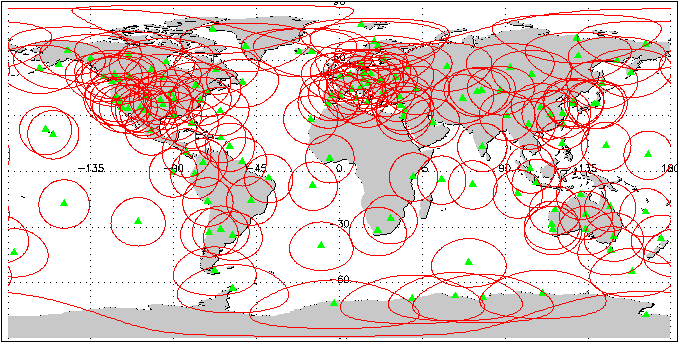
\includegraphics[width=0.95\linewidth]{Ionosphere/figures/gps_sitemap.png}
\caption{Global Map of GPS Network stations used for the quasi-real time maps of $TEC$ available online at iono.jpl.nasa.gov}
\label{Fig:gps_stat}
\end{center}
\end{figure}

\begin{figure}[htb]
\centering
\begin{minipage}[b]{0.48\textwidth}
\centering
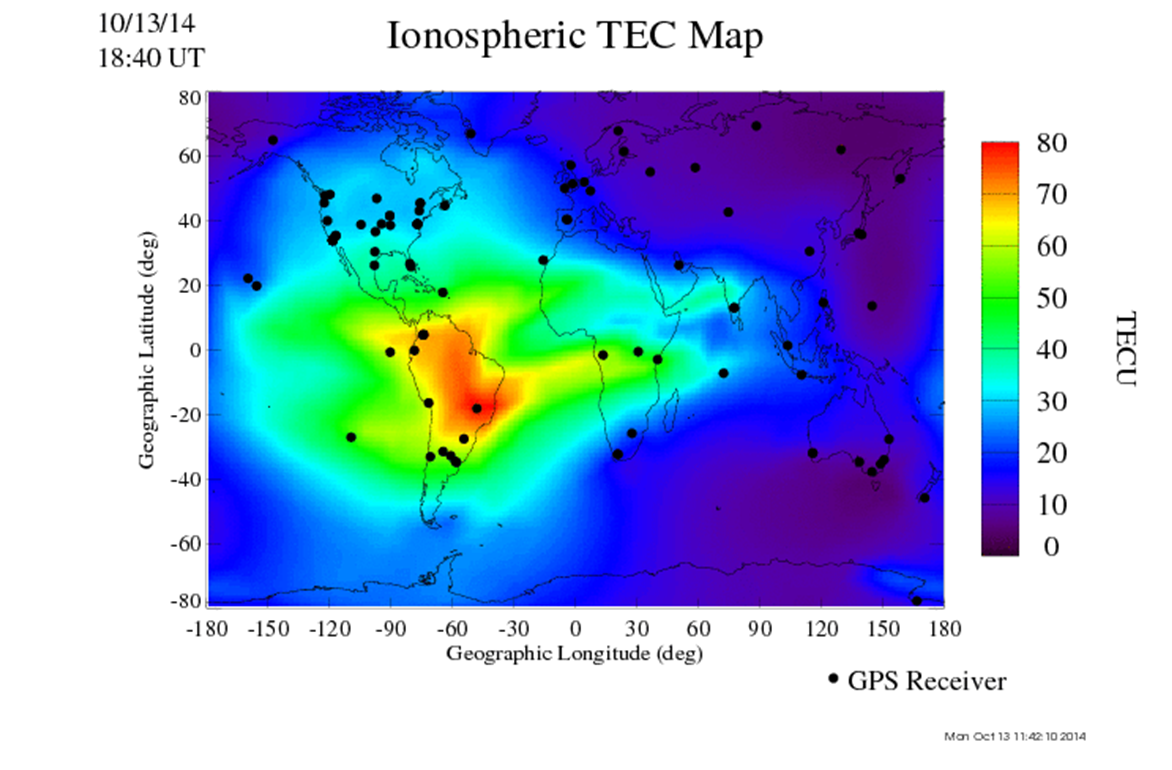
\includegraphics[width=0.95\linewidth]{Ionosphere/figures/TEC_map_20141013_18-40UT.png}
\caption{$TEC$ map for October 13th, 2014 at 18:40 UTC. (Image found at iono.jpl.nasa.gov)  }
\label{Fig:fall_tec_global}
\end{minipage}%
\begin{minipage}[b]{0.02\textwidth}
\hspace{1cm}
\end{minipage}%
\begin{minipage}[b]{0.48\textwidth}
\centering
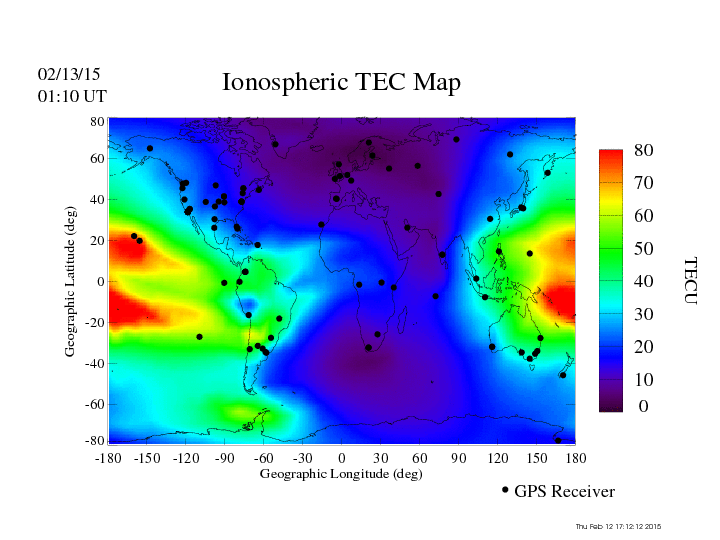
\includegraphics[width=0.95\linewidth]{Ionosphere/figures/TEC_map_20150213_01-10UT.png}
\caption{$TEC$ map for February 13th, 2015 at 01:10 UTC. (Image found at iono.jpl.nasa.gov)  }
\label{Fig:winter_tec_global}
\end{minipage}
\end{figure}


\subsection{Measuring $TEC$}

Real time maps of $TEC$ over the entire world are made by NASA JPL using the GPS stations shown in Figure \ref{Fig:gps_stat} and are available online\footnote{\url{http://iono.jpl.nasa.gov/latest_rti_global.html}}. The plots are based on a five minute average, and the image is updated online every five minutes. 

Example $TEC$ maps for two different times of day (and year) are shown in Figures \ref{Fig:fall_tec_global} and \ref{Fig:winter_tec_global}.  The bright regions with high $TEC$ correspond to the part of the globe currently receiving sunlight at the time the data was collected. Areas close to the equator have much higher $TEC$ than areas near the poles in both the day and night regions.

\begin{figure}[htb]
\centering
\begin{minipage}[b]{0.48\textwidth}
\centering
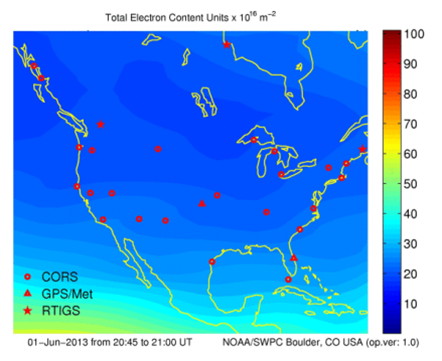
\includegraphics[width=0.95\linewidth]{Ionosphere/figures/NA_TEC_day.png}
\caption{North American TEC map for June 1st, 2013 at 21:00 UTC. (Image found at www.swpc.noaa.gov)   }
\label{Fig:day_TEC_NA}
\end{minipage}%
\begin{minipage}[b]{0.02\textwidth}
\hspace{1cm}
\end{minipage}%
\begin{minipage}[b]{0.48\textwidth}
\centering
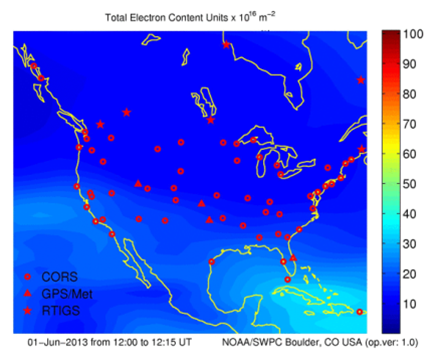
\includegraphics[width=0.95\linewidth]{Ionosphere/figures/NA_TEC_night.png}
\caption{North American TEC map for June 1st, 2013 at 12:15 UTC. (Image found at www.swpc.noaa.gov) }
\label{Fig:night_TEC_NA}
\end{minipage}
\end{figure}

North American $TEC$ maps are also generated by the Space Weather Prediction Center of the National Oceanic and Atmospheric Administration (NOAA)\footnote{\url{http://www.swpc.noaa.gov/products/us-total-electron-content}}. Beyond the regularly updated images, NOAA makes the most recent data ($\sim 24-72 hrs$) available for easy download. Plots of North American $TEC$ for the Isla Guadalupe deployment in June 2013 are shown in Figures \ref{Fig:day_TEC_NA} and \ref{Fig:night_TEC_NA}. 

\begin{figure}[htb]
\begin{center}
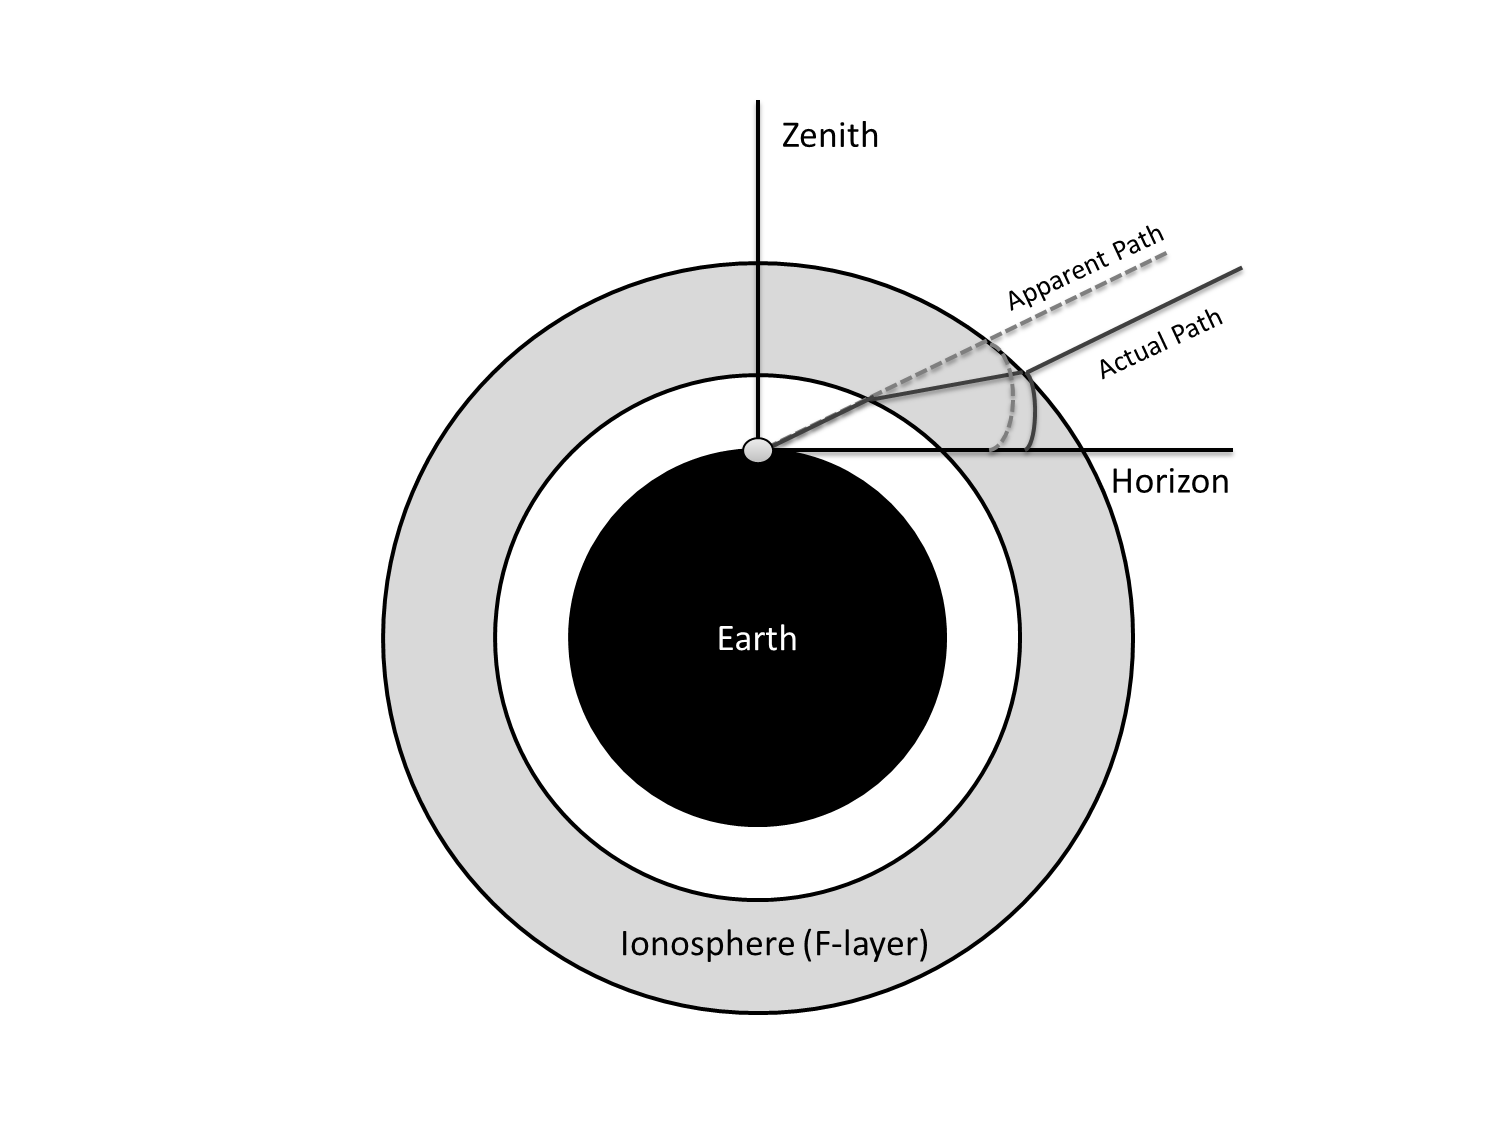
\includegraphics[width=0.95\linewidth]{Ionosphere/figures/refraction.png}
\caption{Ray tracing for incident light with a single ionospheric layer. Sizes are not to scale. }
\label{Fig:iono_refrac}
\end{center}
\end{figure}



\section{Ionospheric Impacts}


\subsection{Refraction}

From basic optics, Snell's law tells us that radiation passing through an interface between materials having different indices of refraction will be bent. The magnitude of this bending depends only on the difference between the indices of the two materials and the incidence angle of the radiation ($n_0 sin \theta_0 = n_1 sin \theta_1$). If radiation passes through a flat plane of material with index $n_1$, having air ($n=1$) on either side, the angle of the radiation coming out the other side of the material is unchanged. However, the ionosphere is a set of spherical layers rather than a flat plane, leading to changes in the angle of the radiation \cite{thompson_2001}. 

Therefore, when radiation enters the ionosphere at some angle $\theta_0 \neq 0$, the radiation reaches the ground with an apparent incidence angle that differs from its arriving incidence angle. This is shown in Figure \ref{Fig:iono_refrac}, where I've used a single ionospheric layer for simplicity. We can define the deflection angle $\delta \theta = \theta_{apparent}-\theta_{actual}$ \cite{thompson_2001}.


\begin{figure}[htb]
\begin{center}
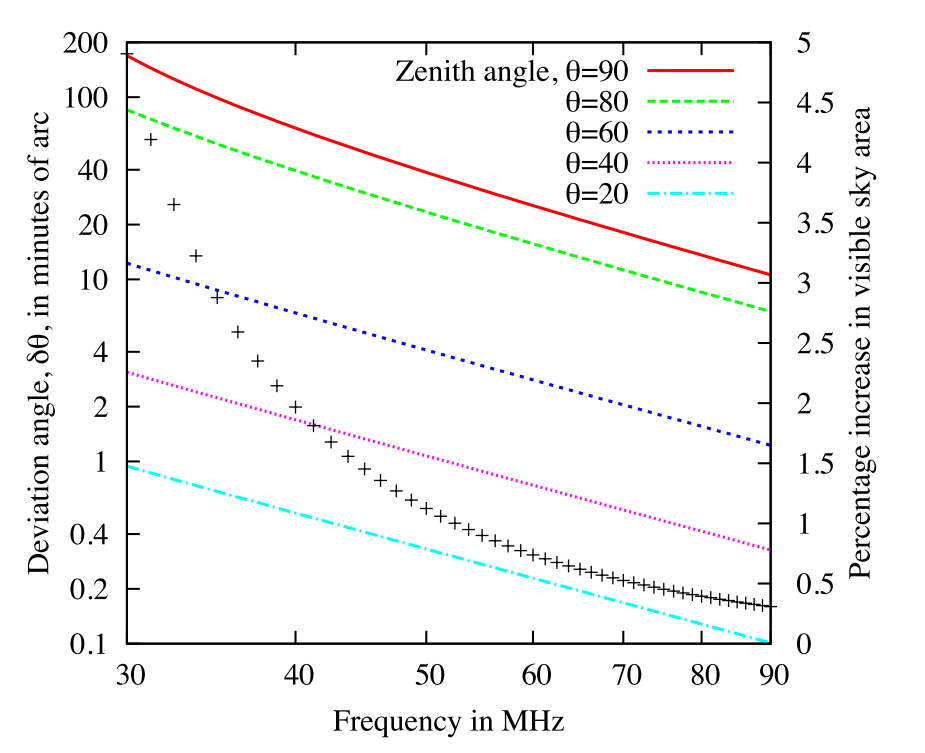
\includegraphics[width=0.85\linewidth]{Ionosphere/figures/refraction_impact.jpg}
\caption{Refraction angle ($\delta \theta$) for $TEC= 10 TECU$ as a function of zenith angle and frequency from Vedantham et al \cite{vedantham_2014}. The predicted level of refraction due to the Earth's ionosphere is below the detection limit of the SCI-HI data collected in June 2013.} 
\label{Fig:refrac_est}
\end{center}
\end{figure} 

To compute $\delta \theta$ requires a model for the ionosphere. The simplest approximation is a single ionospheric layer with constant $n_e$. Using this approximation, $\delta \theta \propto \nu^{-2} cos(\theta)(sin^2 \theta + 2 h_F/R_e)^{-1.5}$, where $h_F$ is the mean height of the ionosphere and $R_e$ is the Earth's radius. Vedantham et al \cite{vedantham_2014} used this approximation, assuming that the total electron content was $10 TECU$ and $h_F = 300 km$, to calculate the deviation angle $\delta \theta$ and percentage increase in visible sky area (beyond the normal horizon), as shown in Figure \ref{Fig:refrac_est}. 


\subsection{Absorption}

Radiation passing through Earth's ionosphere can also be absorbed due to collisions between electrons and other particles in the atmosphere. Most of this absorption will occur at the lowest level of the ionosphere (D-layer) where the number of neutral particles is largest. Absorption is small for $\nu \gg \nu_p$, on the order of 1-2\% \cite{vedantham_2014}. In addition, absorption is frequency dependent and $\propto \nu^{\alpha -2}$, where $\alpha$ is the spectral index of the radiation from the sky \cite{vedantham_2014}. 



\section{Earth's Ionosphere and the SCI-HI system}

Both refraction and absorption due to the ionosphere have the potential to affect the SCI-HI experiment. Refraction will appear as a change in antenna beam pattern compared to the ionosphere-free pattern, while absorption will appear as a multiplicative loss factor that adds additional frequency structure to the data. 

Ionospheric impacts can be assessed and mitigated through two strategies. The first strategy is collection of supplemental data to quantify the expected ionospheric impact. The strategy uses a time dependent estimate of $TEC$ at the SCI-HI deployment site and a good model for absorption and refraction given $TEC$. This allows calculation of $\delta \theta$ and an absorption attenuation factor. $TEC$ estimates can be sourced from publicly available data such as the NASA JPL and NOAA libraries. 

The second strategy is to decrease the ionospheric impact on the data to below \cm signal levels. This decrease requires data that is collected during low $TEC$ times and in low $TEC$ locations. Limiting analysis to data collected during the night will greatly decrease average $TEC$ and ionospheric impacts in the data. In addition, usage of a polar latitude site such as Marion Island, see Figure \ref{Fig:site_map_south}, will help to further decrease average $TEC$.
